\documentclass{../cpct/ctpro}

\title
{
    ACM 算法与微应用开发实验室 21 届成员选拔赛\par
    暨 2021 年 10 月月赛题目
}
\date{2021 年 11 月 6 日}

\begin{document}

\maketitle
\addproblem{K 素数筛}{3000}{256}{传统}{Tifa}
\addproblem{天马行空}{1000}{256}{传统}{AgOH}
\addproblem{双端队列}{1000}{256}{传统}{AgOH}
\addproblem{水的体积}{1000}{256}{传统}{AgOH}
\addproblem{棋牌室}{1000}{256}{传统}{Tifa}
\addproblem{倍思亲}{1000}{256}{传统}{AgOH}

\section*{比赛信息}

\ctinfotab{ACM 个人赛}{C/C++,~Python,~Java}{3}

\section*{题目概况}

\problemtab

\section*{编译命令}

参见 OJ 帮助

\section*{注意事项}

\begin{itemize}
    \item C/C++ 中函数 \verb|main()| 的返回值类型必须是 \verb|int|,程序正常结束时的返回值必须是 $0$。
    \item C/C++ 代码必须完全符合 GNU C/C++ 标准,不能使用诸如绘图、Win32API、中断调用、硬件操作或与操作系统相关的API。
    \item C/C++ 代码中允许使用 STL 类库。
\end{itemize}

\paragraph*{} 祝大家取得好成绩!

\makeproblem
\section*{题目描述}

Tifa:对给定的 $n$,如何快速地在 $[1,n]$ 中筛出所有的素数?

AgOH:这不有手就行?看我表演一波线性筛素数……

Tifa:那如果将恰好能表示为 $k$ 个素数乘积的数称为 $k$-素数, 对给定的 $n,k$,如何快速地在 $[1,n]$ 中筛出所有的 $k$-素数?

AgOH:???

Tifa:那如果将恰好能表示为 $k$ 个\textbf{不同}素数乘积的数称为完全 $k$-素数,对给定的 $n,k$,如何快速地在 $[1,n]$ 中筛出所有的完全 $k$-素数?

AgOH:??????……不慌,实验室的成员们应该能帮我解决这个问题,我先去问问他们去(

\section*{输入格式}

多组数据。

第一行为一个整数 $t~(1\leq t\leq 10^3)$,表示数据组数。

接下来 $t$ 行每行有两个整数 $n~(1 \leq n \leq 2 \times {10}^6),~k~(0 \leq k \leq n)$,含义同描述。

\section*{输出格式}

每组数据输出两行, 其中第一行输出 $k$-素数的结果,第二行输出完全 $k$-素数的结果。

每行首先输出一个数 $m$,表示 $[1,n]$ 中所有 $k$-素数/完全 $k$-素数的个数。

若 $m$ 为 $0$,则结束该行的输出。

若 $m$ 不为 $0$,则接下来隔一个空格后输出一个数 $x$,为 $[1,n]$ 中所有 $k$-素数/完全 $k$-素数的\textbf{异或和}。

\begin{quote}
    \textbf{异或和}:设所有 $k$-素数为 $p_1,p_2,\cdots,p_i$,则它们的异或和 $=p_1 \ xor \ p_2 \ xor \cdots xor \ p_i$,其中 $xor$ 代表异或。
\end{quote}

\section*{输入输出样例}

\testcasetab
{
    4\par
    1 1\par
    20 1\par
    10 2\par
    30 3
}
{
    0\par
    0\par
    8 7\par
    8 7\par
    4 1\par
    2 12\par
    7 27\par
    1 30
}

\makeproblem
\section*{题目描述}

弈缘棋社每年一度的新生赛马上就要开始了!作为弈缘棋社象棋水平最低的棋手的 AgOH 为了不暴露自己的真实实力,设置了一个问题,只有答出这个问题的人才能在象棋盘上吊打 AgOH 一番。问题如下:

给定中国象棋棋盘上的两个点 $p1(x1,y1),p2(x2,y2)$,马从 $p1$ 走到 $p2$ 最少需要多少步呢?

作为参赛棋手的小 T 非常想要赢 AgOH 一盘棋,可他实在做不出毒瘤 AgOH 出的这道题目,于是他马上来求助你,你能帮帮他吗?

注:中国象棋中棋子“马”的行动规则(不考虑蹩马腿):每步一直一斜,即先横着或直着走一格,然后再斜着走一个对角线,俗称“马走日”。棋子不能走出棋盘。如图所示的 $8$ 个绿点为 $(4,7)$ 位置上的马的行动范围。

\begin{center}
    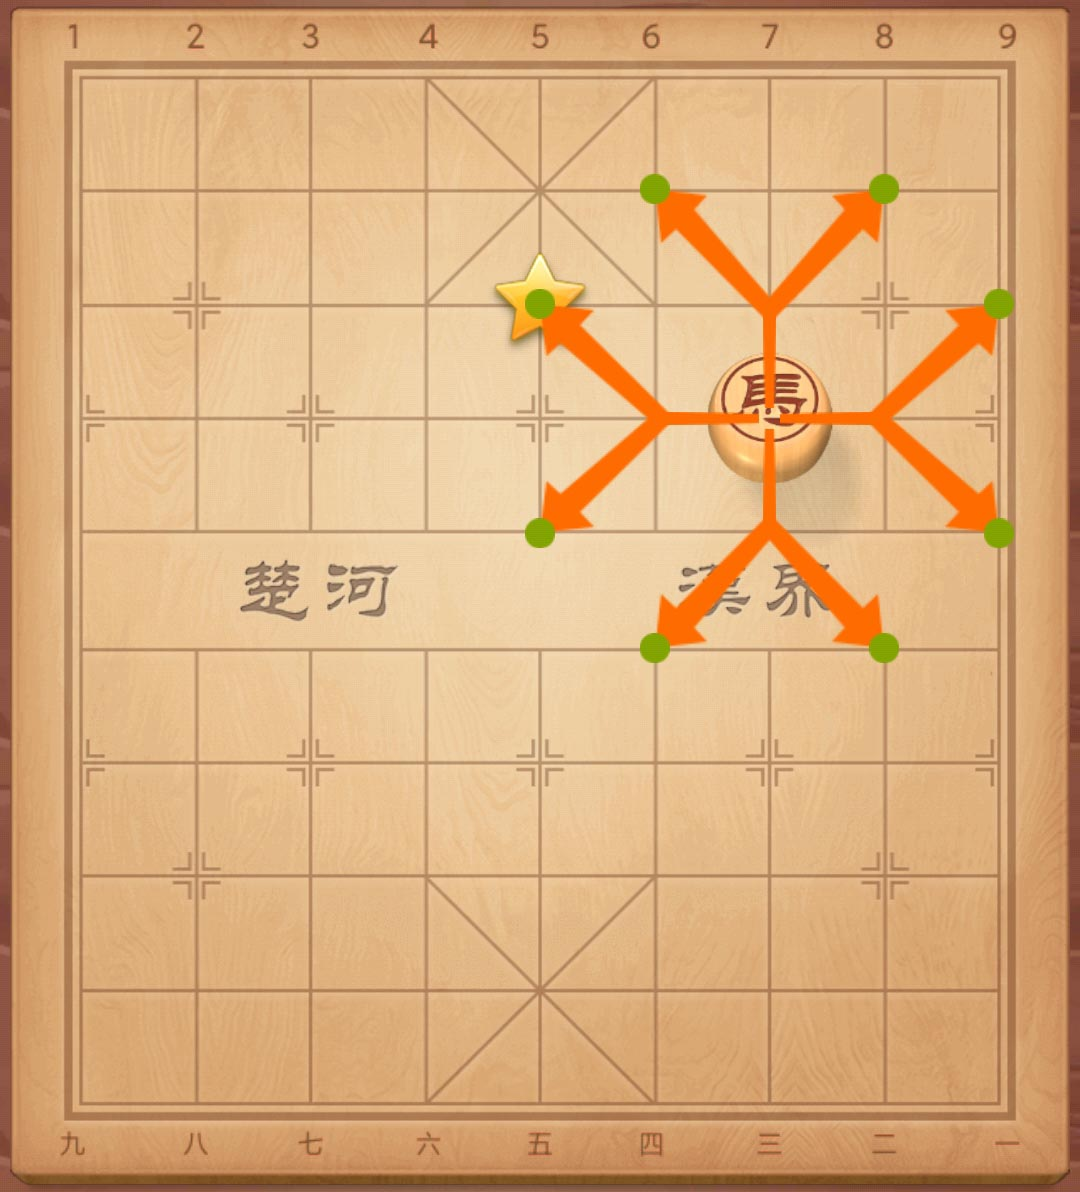
\includegraphics[scale=0.1]{images/chess.jpg}
\end{center}

\section*{输入格式}

一行,四个整数 $x_1,y_1,x_2,y_2~(1 \leq x_1,x_2 \leq 10,~1 \leq y_1,y_2 \leq 9)$。

\section*{输出格式}

一行,一个整数:若马能从 $p1$ 走到 $p2$,输出马从 $p1$ 走到 $p2$ 最少需要多少步;否则输出 $-1$。

\section*{输入输出样例}

\testcasetab
{
    1 1 2 3
}
{
    1
}

\testcasetab
{
    5 5 5 5
}
{
    0
}

\testcasetab
{
    8 5 10 8
}
{
    3
}

\makeproblem
\section*{题目描述}

双端队列是一种常用的数据结构,其支持四种操作:在队头插入一个元素、在队尾插入一个元素、弹出队头的元素、弹出队尾的元素。(弹出:即将元素从双端队列中拿走)

给你一个存放有 $1 \sim n$ 的\textbf{一个排列}的双端队列,你可以对其进行若干次弹出操作(可以弹出队头或队尾),且弹出的元素按弹出顺序排列出的数列必须为递增的,请问最多可以弹出多少个元素?

例如:如下双端队列最多可以弹出 $4$ 个元素,操作顺序为弹出队首元素 $2$、弹出队尾元素 $3$、弹出队尾元素 $4$、弹出队尾元素 $5$。

\begin{center}
    \begin{tabularx}{200pt}{M|M|M|M|M}
        \toprule
        2 & 1 & 5 & 4 & 3 \\
        \bottomrule
    \end{tabularx}
\end{center}

\section*{输入格式}

第一行,一个整数 $n~(1 \leq n \leq 5 \times {10}^5)$。

第二行,$n$ 个整数,代表初始的双端队列。

\section*{输出格式}

一行,一个整数,代表最多能弹出多少个数字。

\section*{输入输出样例}

\testcasetab
{
    5\par
    2 1 5 4 3
}
{
    4
}

\testcasetab
{
    7\par
    1 3 5 6 7 4 2
}
{
    7
}

\makeproblem
\section*{题目描述}

有 $n$ 个矿泉水瓶,第 $i$ 个瓶子里装有 $a_i$ ml 水。

AgOH 会对你进行 $m$ 次询问,每次询问一个区间 $[l,r]$,请你告诉 AgOH 第 $l$ 个瓶子到第 $r$ 瓶子之间(包含第 $l$ 个和第 $r$ 个)的所有瓶子里共装有多少 ml 的水。

\section*{输入格式}

第一行,两个整数 $n,m~(1 \leq n,m \leq {10}^5)$。

第二行,$n$ 个整数 $a_i~(1 \leq a_i \leq 550)$。

第三到第 $m+1$ 行,每行两个整数 $l,r~(1 \leq l \leq r \leq n)$。

\section*{输出格式}

共 $m$ 行,第 $i$ 行代表第 $i$ 次询问的答案。

\section*{输入输出样例}

\testcasetab
{
    5 3\par
    1 2 3 4 5\par
    1 2\par
    2 4\par
    1 5
}
{
    3\par
    9\par
    15
}

\makeproblem
\newcommand{\mahjong}[1]{\raisebox{-.4\height}{\includegraphics[scale=0.5]{images/mahjong/#1.png}}}
\section*{题目描述}

本次比赛实验室内座位布局方式参考……打麻将。

既然都坐成了棋牌室的样子了,不打打麻将实在是说不过去。

当然比赛过程中打一局完整的麻将是不现实的,你只需要判断一副手牌是否是和牌即可。

\begin{quote}
    \hspace{0.15cm} 和牌规则:对于手中的14张手牌,和牌需达成以下条件:

    \begin{itemize}
        \item 有一个雀头;
        \item 有四个面子;
        \item 雀头和各个面子间没有交叉的牌。
    \end{itemize}

    \begin{quote}
        雀头:两张同样的牌,如 \mahjong{1s} \mahjong{1s};

        面子:包括刻子和顺子(不要问为啥没杠,莫抬杠):

        \begin{itemize}
            \item 刻子:三张同样的牌,如 \mahjong{1m} \mahjong{1m} \mahjong{1m};
            \item 顺子:三张相邻的同类型牌(只包括条/索、饼/筒、万三种),如 \mahjong{1m} \mahjong{2m} \mahjong{3m}。

                  \begin{remark}
                      \mahjong{1m} 与 \mahjong{9m}、\mahjong{1p} 与 \mahjong{9p}、\mahjong{1s} 与 \mahjong{9s} 不算作相邻。
                  \end{remark}
        \end{itemize}
    \end{quote}
\end{quote}

\section*{输入格式}

第一行,一个整数 $t$,代表共有 $t$ 组数据。

第 $2 \sim t+1$ 行,每行 $14$ 个用空格分隔开的双字符字符串,代表一副手牌。手牌表示规则如下:

\begin{itemize}
    \item 一个 $1 \sim 9$ 的数字 $x+$ 一个小写字母 $b$,代表 $x$ 饼(也叫 $x$ 筒)。例如 $2b$ 代表 \mahjong{2p}。
    \item 一个 $1 \sim 9$ 的数字 $x+$ 一个小写字母 $t$,代表 $x$ 条(也叫 $x$ 索)。例如 $8t$ 代表 \mahjong{8s}。
    \item 一个 $1 \sim 9$ 的数字 $x+$ 一个小写字母 $w$,代表 $x$ 万。例如 $5w$ 代表 \mahjong{5m}。
    \item 一个 $1 \sim 7$ 的数字 $x+$ 一个小写字母 $z$,从 $1z \sim 7z$ 分别代表 \mahjong{1z}、\mahjong{2z}、\mahjong{3z}、\mahjong{4z}、\mahjong{5z}、\mahjong{6z}、\mahjong{7z}。
\end{itemize}

数据保证只会出现以上样式的牌。与正常的一副麻将不同,每张牌的出现次数\textbf{不限},例如可能出现 14 张白的情况,且这种情况是和牌。

\section*{输出格式}

共 $t$ 行,第 $i$ 行代表第 $i$ 组数据的答案:若该组牌为和牌,输出 \texttt{Tsumo!};反之输出 \texttt{Waiting for Tsumo!}。

\section*{输入输出样例}

\testcasetab
{
    2\par
    1w 2w 3w 4b 5b 6b 7t 8t 9t 1b 1b 1z 2z 6z\par
    1w 2w 3w 4b 5b 6b 7t 8t 9t 1b 1b 2z 2z 2z
}
{
    Waiting for Tsumo!\par
    Tsumo!
}

\section*{说明/提示}

【样例解释】

第一副手牌为:

\begin{center}
    \mahjong{1m} \mahjong{2m} \mahjong{3m} \mahjong{4p} \mahjong{5p} \mahjong{6p} \mahjong{7s} \mahjong{8s} \mahjong{9s} \mahjong{1p} \mahjong{1p} \mahjong{1z} \mahjong{2z} \mahjong{6z}
\end{center}

第二副手牌为:

\begin{center}
    \mahjong{1m} \mahjong{2m} \mahjong{3m} \mahjong{4p} \mahjong{5p} \mahjong{6p} \mahjong{7s} \mahjong{8s} \mahjong{9s} \mahjong{1p} \mahjong{1p} \mahjong{2z} \mahjong{2z} \mahjong{2z}
\end{center}

\makeproblem
\section*{题目描述}

\begin{center}
    
\includegraphics[scale=0.5]{images/God.png}
\end{center}

干员异客的攻击方式为:“攻击造成\textbf{法术伤害},且会在 $4$ 个敌人间跳跃,每次跳跃伤害降低 $15 \%$ 并造成短暂停顿”。即:若敌人被击中时,当前攻击已经击中了 $i$ 个人,则该攻击会对其造成 $(85 \%)^i$ 倍的\textbf{法术伤害}。

法术伤害会受到敌人\textbf{法抗}的百分比削减,即若对一个\textbf{法抗}为 $p \%$ 的敌人造成 $s$ 点法术伤害,该敌人仅会受到 $s \times (1-p \%)$ 点\textbf{真实伤害}。

假设敌人具有无限点血量,给出异客的攻击力和四个被击中的敌人的法抗,请你计算出异客一次攻击对所有敌人共造成了多少\textbf{真实伤害}。

注意:因为敌人的血量为整数,所以对\textbf{每个敌人}打出的真实伤害都需要向下取整。因浮点误差影响,所输出答案与真实答案之间允许有 $2$ 以内的误差。

\section*{输入格式}

第一行,一个整数 $t~(1 \leq t \leq {10}^5)$,代表共有 $t$ 组数据。

第 $2 \sim t+1$ 行,每行 $5$ 个整数,分别代表异客的攻击力 $A~(1 \leq A \leq 1500)$ 和依次被击中的 $4$ 个敌人的法抗 $p_1,p_2,p_3,p_4~(0 \leq p_i \leq 100)$。

\section*{输出格式}

共 $t$ 行,第 $i$ 行代表第 $i$ 组数据的答案。

\section*{输入输出样例}

\testcasetab
{
    3\par
    1000 20 20 20 20\par
    1500 10 20 30 40\par
    1001 25 33 37 70
}
{
    2549\par
    3680\par
    1959
}

\end{document}
